\documentclass[11pt,a4paper]{article}
\usepackage[margin=1in]{geometry}
\usepackage[T1]{fontenc}
\usepackage[utf8]{inputenc}
\usepackage{lmodern}
\usepackage{booktabs}
\usepackage{longtable}
\usepackage{graphicx}
\usepackage{float}
\usepackage{hyperref}
\usepackage{setspace}
\usepackage{enumitem}
\usepackage{amsmath}

\title{Semester Project: Domain Discovery, Recommendation, and Graph Intelligence\\
\large Milestone: Recommendation, Ranking, and Predictive Decision Engine (Week 10)}
\author{Iam Anthony Marcelo Alvarez Orellana \\ Jeffrey Ulises Diaz Villanueva \\ Paula Jimena Mancilla Cienfuegos \\ Fernando Samuel Paredes Espinoza}
\date{}

\begin{document}
\maketitle
\onehalfspacing

\section{Task Framing}

\textbf{Task type:} Recommendation.

Given a user's positive interaction history (games endorsed via \texttt{voted\_up=True}), the system predicts which unseen game that user would also endorse. The output is a ranked list of candidate games.

This is a \textbf{personalized recommendation} problem: the unit being recommended is a Steam game, the unit of personalization is the user interaction history, and the quality signal is the recovered hold-out positive interaction.

The clustering results from Week 7 (six semantic segments: Casual, Action, Local Multiplayer, Narrative/JRPG, VR, Strategy) feed into this pipeline. A user's interaction history implies a probable cluster affinity, making this a \textbf{segmentation-feeding-recommendation} architecture.

\section{Data Alignment}

All systems operate on the same 500-game universe from \texttt{data/processed/steam\_v1.parquet}. \texttt{AppID} is the common join key:

\begin{itemize}[leftmargin=*]
  \item \texttt{steam\_v1.parquet} --- user interaction records (\texttt{author\_steamid}, \texttt{AppID}, \texttt{voted\_up}, \texttt{author\_playtime\_forever})
  \item \texttt{games\_may2024\_full.csv} --- game metadata (\texttt{name}, \texttt{tags}, \texttt{genres}, \texttt{categories}, \texttt{short\_description}, \texttt{recommendations})
  \item \texttt{artifacts/clustering/cluster\_labels\_k6.npy} --- cluster labels from Week 7
\end{itemize}

Alignment is exact by construction: the parquet was built via an inner join on \texttt{AppID} in \texttt{src/ingest.py}.

\section{Evaluation Protocol}

\begin{itemize}[leftmargin=*]
  \item \textbf{Interaction matrix:} Sparse binary matrix, users $\times$ games. Value = 1 when \texttt{voted\_up = True}. Duplicates de-duplicated before construction.
  \item \textbf{Qualifying users:} Users with $\geq 2$ distinct positive interactions (minimum one training + one hold-out).
  \item \textbf{Train/test split:} For each qualifying user, one positive interaction is randomly held out (\texttt{random\_state=42}). Remaining interactions form the training set.
  \item \textbf{Candidate pool:} All games the user has NOT interacted with in training (full game universe minus known positives).
  \item \textbf{Primary metric:} Hit-Rate at 10 (HR@10) --- fraction of qualifying users for whom the held-out game appears in their top-10 recommendations.
  \item \textbf{Leakage prevention:} Training items masked to $-\infty$ before ranking. The held-out item is never used during training or score computation.
\end{itemize}

\textbf{Dataset statistics:}
\begin{itemize}[leftmargin=*]
  \item Positive interactions: 442,652
  \item Unique users: 426,601 | Unique games: 484
  \item Qualifying users (hold-out evaluation): 12,389
\end{itemize}

\section{Baseline 1 --- Popularity}

\textbf{Design:} All games ranked by aggregate \texttt{recommendations} count. Every user receives the same ranking. No personalization.

\textbf{Justification:} Establishes the non-personalized ceiling. Any personalized system failing to beat popularity is unjustified in complexity.

\textbf{Limitation:} Biases strongly toward well-known AAA titles; cannot surface niche Indie games.

\section{Baseline 2 --- Content-Based}

\textbf{Design:} TF-IDF on \texttt{name + short\_description + tags + genres + categories} (1--2 grams, 3,000 features). \texttt{TruncatedSVD} reduces to 50 latent components. User vector = centroid of training game vectors. Ranking by cosine similarity.

\textbf{Justification:} Cold-start friendly; interpretable similarity (games scored high if they share tag/description vocabulary).

\textbf{Limitation:} Overspecializes to user's known preferences; ignores collective behavioral signal.

\section{System 3 --- Matrix Factorization (SGD)}

\textbf{Objective:}
\begin{equation}
\min_{P,Q} \sum_{(u,i) \in \Omega} \left(R_{ui} - p_u^\top q_i\right)^2 + \lambda \left(\|P\|_F^2 + \|Q\|_F^2\right)
\end{equation}

where $R \in \{0,1\}^{m \times n}$ is the binary interaction matrix, $\Omega$ is the set of observed positive pairs, $P \in \mathbb{R}^{m \times k}$ are user latent factors, and $Q \in \mathbb{R}^{n \times k}$ are item latent factors.

\textbf{SGD update rules per observed pair $(u, i)$:}
\begin{align}
p_u &\leftarrow p_u + \eta\,(e_{ui}\, q_i - \lambda\, p_u) \\
q_i &\leftarrow q_i + \eta\,(e_{ui}\, p_u - \lambda\, q_i)
\end{align}
where $e_{ui} = R_{ui} - p_u^\top q_i$.

\textbf{Hyperparameters:}

\begin{longtable}{p{0.22\linewidth}p{0.15\linewidth}p{0.55\linewidth}}
\toprule
\textbf{Parameter} & \textbf{Value} & \textbf{Justification} \\
\midrule
Learning rate $\eta$ & 0.03 & Standard for implicit binary data; larger values cause divergence \\
Regularization $\lambda$ & 0.01 & Controls factor scale; prevents overfitting on 99.8\% sparse matrix \\
Epochs & 30 & Sufficient for convergence in 500-game universe \\
Latent dim $k$ & \{10, 20, 50\} & Swept via HR@10; best $k$ used for final model \\
Init & $\mathcal{N}(0, 0.1^2)$ & Small random values to break symmetry \\
\bottomrule
\end{longtable}

\section{System 4 --- Hybrid Recommender}

\textbf{Design:} Weighted linear combination of content and MF scores:
\begin{equation}
s_{\text{hybrid}}(u, g) = \alpha \cdot s_{\text{content}}(u, g) + (1-\alpha) \cdot s_{\text{MF}}(u, g)
\end{equation}

Both scores min-max normalized to $[0,1]$ before combination. $\alpha \in \{0.1, 0.3, 0.5, 0.7, 0.9\}$ swept empirically.

\textbf{Why the hybrid is legitimate:} \texttt{AppID} is the common key for both the content matrix (built from catalog) and the MF item factors (built from interaction parquet). Both systems index games identically --- no cross-catalog alignment issue.

\section{Offline Evaluation Results}

Results generated by \texttt{python src/recommendation.py} with \texttt{random\_state=42}. Full metrics in \texttt{artifacts/recommendation/rec\_metrics.json}.

\begin{longtable}{p{0.30\linewidth}rrr}
\toprule
\textbf{System} & \textbf{HR@5} & \textbf{HR@10} & \textbf{HR@20} \\
\midrule
Popularity baseline & 0.4597 & 0.5796 & 0.7124 \\
Content-based baseline & 0.1806 & 0.2170 & 0.2669 \\
MF $k=10$ & 0.1103 & 0.1888 & 0.2949 \\
MF $k=20$ & 0.0764 & 0.1333 & 0.2183 \\
MF $k=50$ & 0.0756 & 0.1235 & 0.1998 \\
\textbf{Hybrid ($\alpha=0.3$, $k=10$)} & \textbf{0.2057} & \textbf{0.2569} & \textbf{0.3330} \\
\bottomrule
\end{longtable}

\textit{12,389 qualifying users, 484-game universe, hold-out evaluation.}

\begin{figure}[H]
  \centering
  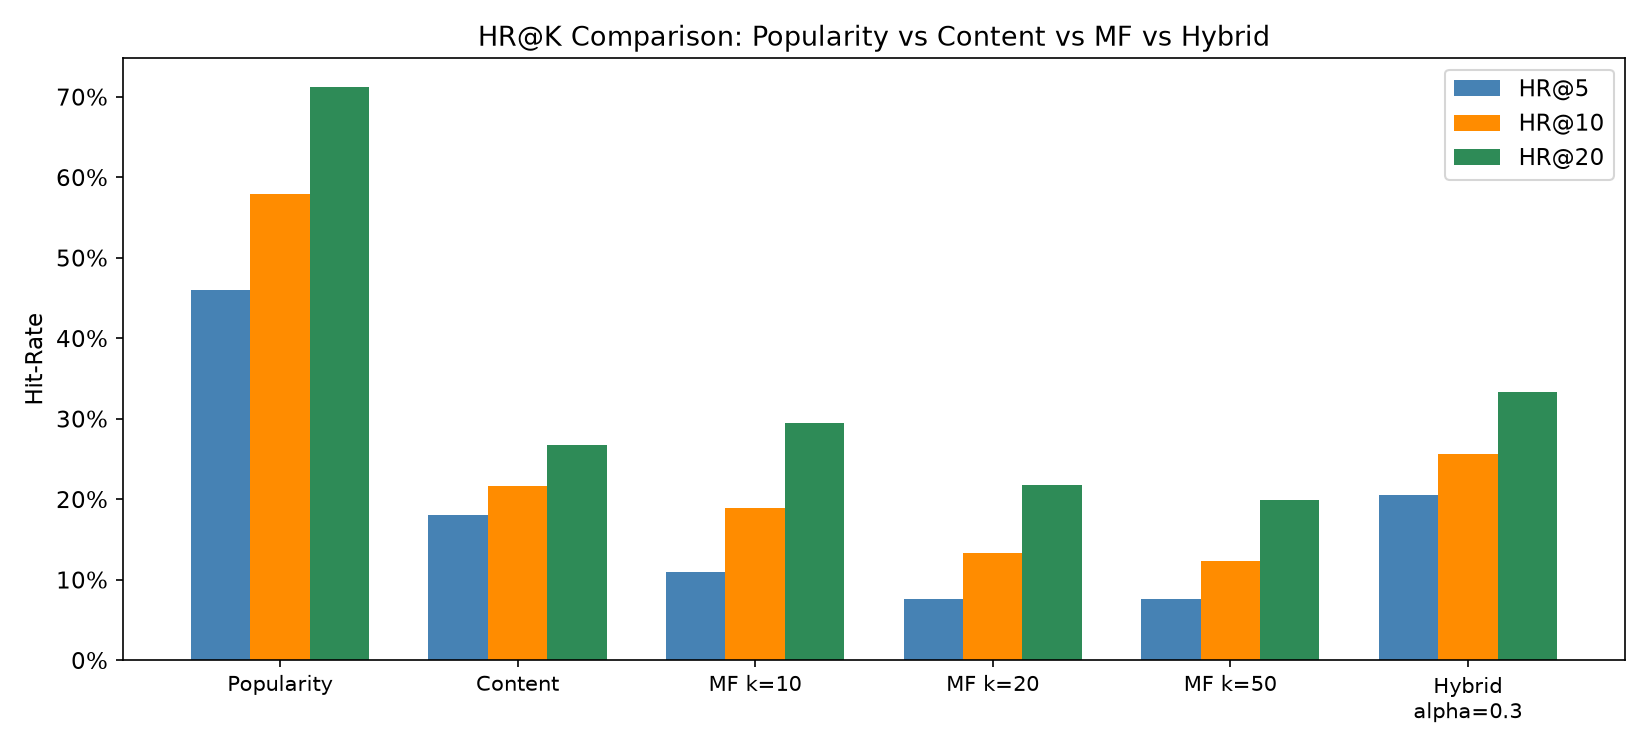
\includegraphics[width=0.95\linewidth]{fig01_hr_comparison.png}
  \caption{HR@K across all systems at $K \in \{5, 10, 20\}$. Popularity dominates due to the small 484-game universe; among personalized systems, the Hybrid ($\alpha=0.3$) achieves the highest HR@10 at 25.7\%.}
\end{figure}

\begin{figure}[H]
  \centering
  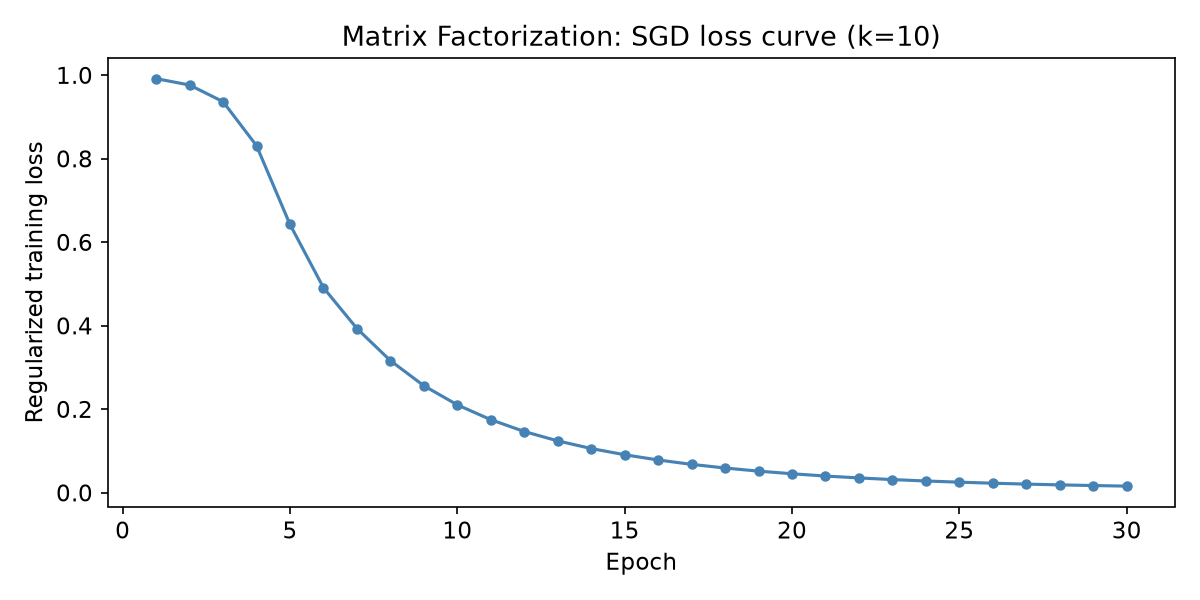
\includegraphics[width=0.80\linewidth]{fig02_mf_loss_curve.png}
  \caption{SGD training loss per epoch for the best MF model ($k=10$). Loss decreases monotonically, confirming convergence within 30 epochs.}
\end{figure}

\begin{figure}[H]
  \centering
  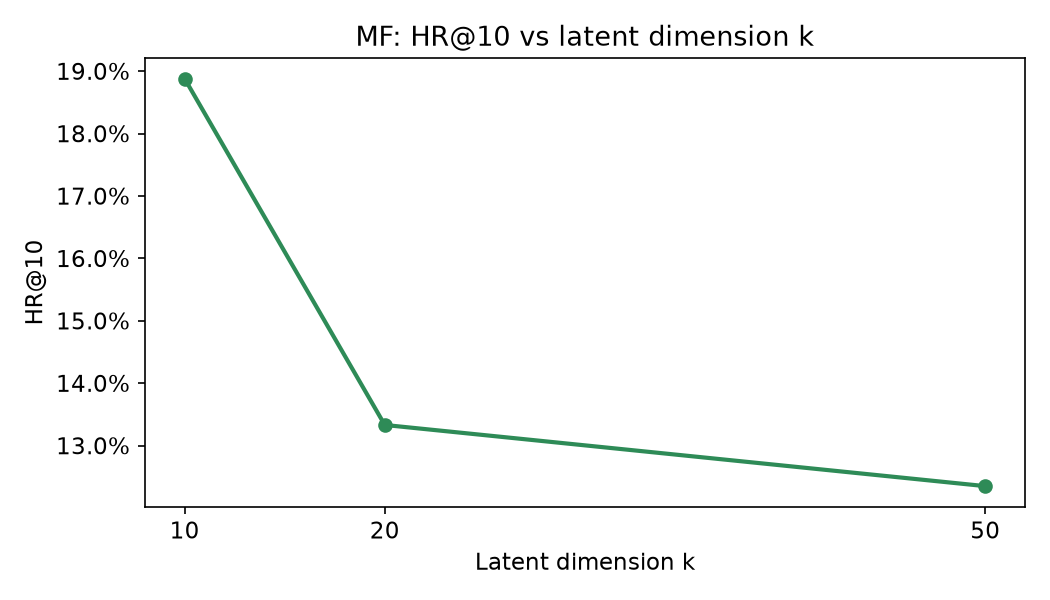
\includegraphics[width=0.70\linewidth]{fig03_mf_k_sweep.png}
  \caption{HR@10 versus latent dimension $k$. Smaller $k=10$ generalizes better on this sparse 484-game universe; higher $k$ overfits the scarce interaction signal.}
\end{figure}

\begin{figure}[H]
  \centering
  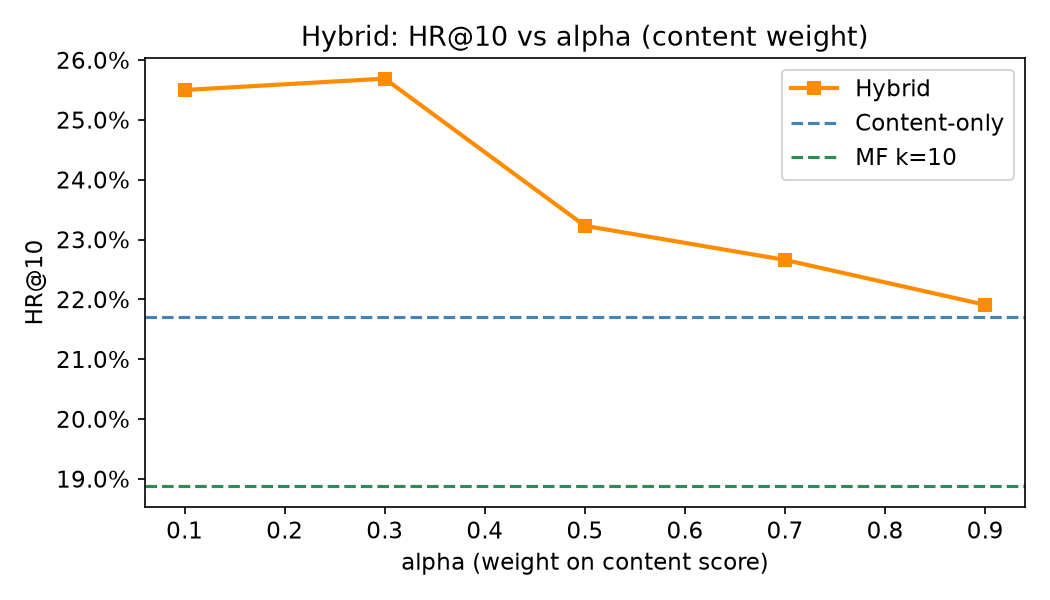
\includegraphics[width=0.70\linewidth]{fig04_hybrid_alpha_sweep.png}
  \caption{Hybrid HR@10 versus content weight $\alpha$. The optimal $\alpha=0.3$ means 30\% content + 70\% MF. Dashed lines show individual system baselines.}
\end{figure}

\section{Error Analysis}

Analysis performed on the best MF model ($k=10$, $\alpha=0.3$ hybrid).

\textbf{Strong cases (hits):} Users whose training history concentrates in a single cluster receive accurate recommendations --- MF identifies users with similar narrow profiles and retrieves their endorsed games.

\textbf{Failure cases (misses):} Most common failure mode is \textbf{cross-cluster taste}: a user's training history spans two or more clusters (e.g., C1 Action and C3 Narrative), but the held-out game belongs to a third cluster. Latent factors average out competing signals and fail to recover the minority interest.

A secondary failure mode is \textbf{popularity contamination}: when MF score is weak (sparse history, only 2 qualifying interactions), the model defaults to broadly popular games rather than the user's specific interest.

\section{Reproducible Pipeline}

\begin{verbatim}
# Step 1 -- Ingestion (if data not already present)
python src/ingest.py

# Step 2 -- Feature engineering
python src/feature_engineering.py

# Step 3 -- Clustering (Week 7)
python src/clustering_week7.py

# Step 4 -- Recommendation engine (produces artifacts/recommendation/)
python src/recommendation.py

# Step 5 -- Generate all report figures
python src/generate_figures.py
\end{verbatim}

All outputs are deterministic with \texttt{random\_state=42}.

\section{Ethics and Access Note}

\begin{itemize}[leftmargin=*]
  \item \textbf{Data provenance:} All interaction data comes from \texttt{steam\_v1.parquet} built by \texttt{src/ingest.py} from the Kaggle Steam reviews dataset (CC0 license).
  \item \textbf{Personal data risks:} \texttt{author\_steamid} is used as a row index. It is treated as an opaque identifier --- no real names, emails, or financial data are involved. Steam IDs are public-facing identifiers on the platform.
  \item \textbf{Recommendation fairness:} Popularity baseline and MF both exhibit popularity bias, recommending widely-reviewed games. This contradicts the product goal of surfacing niche Indie titles. Future work should incorporate inverse propensity scoring to reduce exposure concentration.
\end{itemize}

\end{document}
